\documentclass{article}

\usepackage[utf8]{inputenc}
\usepackage[spanish]{babel}

\usepackage{caratula}

\usepackage{subcaption}
\usepackage{graphicx}
\usepackage{subfig}
\usepackage{dirtytalk}
\usepackage{enumerate}

\usepackage{amssymb}
\usepackage{mathtools}
\usepackage{amsmath}
\usepackage{amsthm}

\usepackage{algorithm}
\usepackage{algpseudocode}
\usepackage{listingsutf8}

\usepackage{float}
\floatplacement{figure}{h!}

\usepackage{geometry}
\usepackage{fixltx2e}
\usepackage{wrapfig}
\usepackage{cite}
\usepackage{dsfont}

\usepackage[space]{grffile}

\geometry{
 a4paper,
 total={210mm,297mm},
 left=30mm,
 right=30mm,
 top=30mm,
 bottom=30mm,
 }
 
\newtheorem{theorem}{Teorema}[section]
\newtheorem{corollary}{Corolario}[theorem]
\newtheorem{lemma}{Lema}[theorem]
 
\theoremstyle{definition}
\newtheorem{definition}{Definición}[section]
 
\theoremstyle{remark}
\newtheorem*{remark}{Observación}
 
\begin{document}
% Estos comandos deben ir antes del \maketitle
\materia{Algoritmos y Estructuras de Datos III} % obligatorio

\titulo{Trabajo Práctico 3}
\subtitulo{}
\grupo{}

\integrante{Bayardo Julián}{850/13}{julian@bayardo.com.ar} % obligatorio
\integrante{Cuneo Christian}{755/13}{chriscuneo93@gmail.com} % obligatorio 
\integrante{Frassia Fernando}{340/13}{ferfrassia@gmail.com} % obligatorio 
\integrante{Gambaccini Ezequiel}{715/13}{ezequiel.gambaccini@gmail.com} % obligatorio 
 
\maketitle

\pagebreak

\tableofcontents

\pagebreak

\section{Sobre la experimentación}

Para verificar la correctitud de los algoritmos de los problemas uno y dos, decidimos generar familias de grafos con números cromáticos conocidos, y armar listas de colores tal que siempre fuera posible colorear los grafos con al menos la cantidad mínima de colores. 
Las familias elegidas fueron estrella, ciclo, rueda, bipartito, completo y árbol binario.
Estas mismas familias, además de grafos aleatorios, se usaron para probar las heurísticas y ver su efectividad, es decir, cuan lejos del óptimo quedaba el resultado de las mismas para un grafo dado.

Estos grafos los generamos a partir de una serie de scripts variando su cantidad de vértices, aristas, variedad de colores, y longitud máxima de la lista de colores. Por ejemplo, al poder elegir la longitud máxima de la lista de colores, pudimos limitar la misma a 2 de longitud para el caso del problema 1 de 2 list coloring.

Para probar los diferentes parámetros, variamos los vértices de 5 a 50, los colores de 4 a n+1, y las aristas de 0 a $\frac{n*(n-1)}{2}$ para las diferentes familias de grafos, y generábamos las instancias válidas para cada familia. Esto termino generando unos 250000 de casos de prueba en total para cada ejercicio de heurísticas y 2 list coloring.
Para backtracking sin podas, redujimos la cantidad de casos de prueba a 1000 aproximadamente, debido a su complejidad exponencial. El backtracking con podas, sin embargo, pudo resolver unos 50000 casos sin problemas.


\section{Problema 1}

El primer problema presenta un grafo a colorear en los que cada nodo tiene solo 1 o 2 colores posibles a elegir. A la hora de resolverlo pensamos reducir este problema a un problema ya resuelto. Para este caso especifico logramos ver que es posible transformar una instancia de este problema a una instancia de 2-Satisfiability.\par
Para conseguir esto necesitamos lograr convertir nuestra instancia en un conjunto de clausulas (que consisten de un OR entre varias variables o sus negaciones) tal que, si hay una asignación de estas variables que haga que todas las clausulas sean verdaderas, significa que nuestra instancia original tiene un coloreo valido. Y también necesitamos poder calcular este coloreo.\smallbreak
Entendiendo esto procedemos a buscar una forma correcta de crear una formula de lógica booleana a partir de una instancia del problema dado.\par
Cada nodo puede ser coloreado con uno o dos colores. 
En el caso que un nodo (llamémoslo A) tenga dos colores (digamos azul y rojo), tendremos las siguientes posibilidades:
\begin{enumerate}
\item A es rojo ($Ar$)
\item A no es rojo ($A\neg r$)
\item A es azul ($Aa$)
\item A no es azul ($A\neg a$)
\end{enumerate}
Naturalmente se deduce que $Ar \implies A\neg a$ y también $A\neg a \implies Ar$ ya que $A$ no puede estar coloreado con dos colores diferentes. Al mismo tiempo se tiene que $Aa \implies A\neg r$ y $A\neg r \implies Aa$ por lo mismo.

\begin{figure}
\centering
\begin{minipage}{0.45\textwidth}
\centering
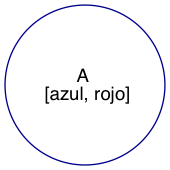
\includegraphics[width=3cm]{graphs/ej1/ej1_intro_2c.png}
\caption{Nodo entrada\label{grf:ex1-example-2c}}
\end{minipage}\hfill
\begin{minipage}{0.45\textwidth}
\centering
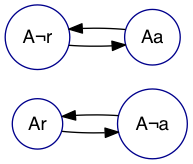
\includegraphics[width=3.5cm]{graphs/ej1/ej1_intro_2c_impl.png}
\caption{Grafo de implicaciones\label{grf:ex1-example-2c_impl}}
\end{minipage}
\end{figure}


En el caso en que tenga solo un color (digamos azul) tenemos las siguientes posibilidades:
\begin{enumerate}
\item A es azul
\item A no es azul
\end{enumerate}
En este caso como es un único color necesitamos que este nodo este coloreado de este único color, por lo tanto la única implicación que siempre resulta en verdad es: $A\neg a \implies Aa$.

\begin{figure}
\centering
\begin{minipage}{0.45\textwidth}
\centering
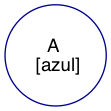
\includegraphics[width=2.5cm]{graphs/ej1/ej1_intro_1c.png}
\caption{Nodo entrada\label{grf:ex1-example-1c}}
\end{minipage}\hfill
\begin{minipage}{0.45\textwidth}
\centering
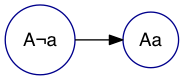
\includegraphics[width=3.5cm]{graphs/ej1/ej1_intro_1c_impl.png}
\caption{Grafo de implicaciones\label{grf:ex1-example-1c_impl}}
\end{minipage}
\end{figure}

Luego, supongamos que hay dos nodos: $A$ que puede colorearse con azul y rojo, y $B$ que puede colorearse con azul. $A$ y $B$ son adyacentes.

Las implicaciones que vimos anteriormente siguen formando parte de la formula general, pero ahora los nodos son adyacentes y comparten un color en la lista de colores azul, por lo tanto tenemos que tener en cuenta que no pueden estar ambos nodos coloreados de este color al mismo tiempo. De esto ultimo generamos unas nuevas implicaciones: $Aa \implies B\neg a$ y $Ba \implies A\neg a$.


\begin{figure}
\centering
\begin{minipage}{0.45\textwidth}
\centering
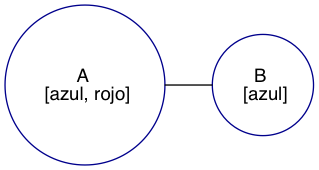
\includegraphics[width=5cm]{graphs/ej1/ej1_intro_2na.png}
\caption{Nodo entrada\label{grf:ex1-example-2na}}
\end{minipage}\hfill
\begin{minipage}{0.45\textwidth}
\centering
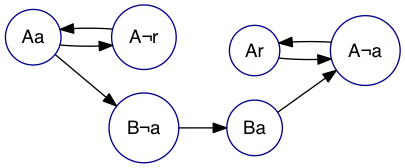
\includegraphics[width=6cm]{graphs/ej1/ej1_intro_2na_impl.png}
\caption{Grafo de implicaciones\label{grf:ex1-example-2na_impl}}
\end{minipage}
\end{figure}

Si en cambio tenemos dos nodos: $A$ que puede colorearse con azul y verde, y $B$ que puede colorearse con rojo, y estos son adyacentes, no habría ninguna implicación mas que tener en cuenta.

\begin{figure}
\centering
\begin{minipage}{0.45\textwidth}
\centering
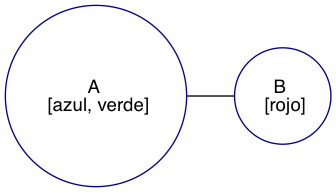
\includegraphics[width=5cm]{graphs/ej1/ej1_intro_2n.png}
\caption{Nodo entrada\label{grf:ex1-example-2n}}
\end{minipage}\hfill
\begin{minipage}{0.45\textwidth}
\centering
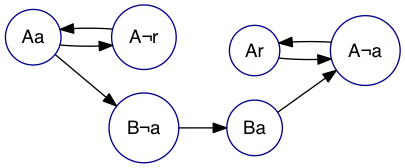
\includegraphics[width=4cm]{graphs/ej1/ej1_intro_2n_impl.png}
\caption{Grafo de implicaciones\label{grf:ex1-example-2n_impl}}
\end{minipage}
\end{figure}

Al llegar a este punto ya tenemos diseñada una forma de crear una formula lógica a partir del grafo de entrada. Como vimos, cada variable de esta formula respresenta un estado especifico de un nodo del grafo de entrada, y al mismo tiempo, las implicaciones entre ellos limitan lo que puede suceder (por ejemplo si un nodo es de un color no puede ser del otro, y viceversa).
Por lo tanto, si asignar un valor a todas estas variables sin llegar a una contradicción en la formula general entonces habremos encontrado un coloreo valido para el grafo de entrada.

Resolver el problema de ver si la formula que encontramos es satisfacible y, si es así, encontrar una asignación valida se resuelve con el procedimiento descripto por Aspvall, Plass y Tarjan en 1979, y fue explicado en clase. Consiste en:
\begin{enumerate}
\item Crear el grafo de implicaciones a partir del grafo de entrada (en nuestro caso utilizando las reglas que vimos anteriormente)
\item Encontrar las componentes fuertemente conexas del grafo de implicaciones.
\item Chequear que no haya una variable y su complemento en una misma componente fuertemente conexa. Si esto sucede la formula no es satisfacible.
\item Construimos el grafo denso de componentes fuertemente conexas.
\item Asignamos un valor a cada componente fuertemente conexa ($true$ o $false$) de forma que no se formen contradicciones y la formula booleana sea verdadera. Al hacer esto al mismo tiempo estamos coloreando el grafo original, ya que le asignamos $true$ o $false$ a cada estado de los nodos originales, y cada estado representaba si un nodo era o no era de un color especifico.
\end{enumerate}

Ahora veamos cada paso mas detalladamente:
\begin{enumerate}
\item Para crear el grafo utilizamos las reglas que describimos anteriormente. Siendo $G=(V,E)$ el grafo de entrada, realizamos un nuevo grafo dirigido de $|V|*4$ vertices, en caso que un nodo sea coloreable con dos colores usara los cuatro nodos nuevos  ($color1,notcolor1, color2, notcolor2$), en caso que sea coloreable con un solo color usara solo dos nodos del nuevo y los otros dos serán marcados como "no utilizados" ($color1,notcolor1,unused,unused$). Esto lo hacemos para poder ubicar en $O(1)$ una variable que representa un estado de un nodo original a partir del numero de nodo original, el numero de color, y un $true$ o $false$.
\item Para encontrar las componentes fuertemente conexas implementamos el algoritmo de Kosaraju, que, dado un grafo dirigido, nos devuelve las componentes fuertemente conexas del grafo en orden topológico inverso. En nuestro caso además de devolver cada componente como una lista de nodos, devuelve un vector que, dado el nodo del grafo de implicaciones almacena el numero de la componente a la que pertenece.
\item Chequear que no haya una variable y su complemento en una misma componente fuertemente conexa es sencillo, iteramos por cada variable del grafo de implicaciones y chequeamos que la variable y su complemento no tengan asignados el mismo numero de componente conexa, utilizando el vector que vimos en el punto anterior.
\item Para construir el grafo denso de componentes fuertemente conexas simplemente creamos un digrafo con cantidad de nodos igual a la cantidad de componentes fuertemente conexas, y luego iteramos por cada nodo del grafo de implicaciones, vemos sus vecinos, y si pertenecen a una componente distinta conectamos estas componentes en la misma dirección que la implicación.
\item En este paso iteramos desde la ultima componente fuertemente conexa (topológicamente hablando) y, si ninguna de sus variables ya tiene asignado un valor de verdad, le asignamos a toda la componente $true$. Al mismo, a medida que le asignamos a cada variable $true$, a su complemento le asignamos $false$. De este modo terminaremos asignando un valor de verdad a cada componente fuertemente conexa (las variables que la componen) y por ende, estaremos coloreando el grafo original.
\end{enumerate}

\subsection{Análisis de complejidad}
Primero evaluemos como sera el tamaño del grafo de implicaciones con respecto al grafo de entrada, ya que la mayoría de las operaciones del algoritmo se realizan sobre el grafo de implicaciones.

El grafo de implicaciones tendrá como mucho 4 veces la cantidad de nodos del grafo original, ya que como vimos anteriormente, si un nodo tiene 2 posibles colores entonces habrá 4 estados en el grafo de implicaciones, y si tiene un color posible habrá 2.

La cantidad de aristas en el grafo de implicaciones no es tan fácil de calcular, pero veamos que tendremos: en el caso de un nodo con un solo color posible, una arista que conecte el estado negativo con el positivo; y en el caso de un nodo con dos colores posibles tendremos una arista que conecte el estado positivo de un color con el negativo del otro color, y el negativo de un color con el positivo del otro, en total 4. Tomemos como cota superior 4 aristas (en el grafo de implicaciones) por cada nodo en el grafo original.
Luego, si dos nodos son vecinos en el grafo original, si no comparten color entonces no habrá ninguna arista que relacione los nodos en el grafo de implicaciones, si en cambio comparten un color habrá 2 aristas que reflejen esto en el grafo de implicaciones, y si comparten 2 colores habrá 4 aristas en el grafo de implicaciones.

En conclusión, tomando siempre cotas superiores, siendo $n$ el numero de vértices del grafo de entrada y siendo $m$ el numero de aristas de este mismo grafo, el grafo de implicaciones tendrá como mucho $n*4$ vértices y $n*4+m*4$ aristas

\begin{algorithm}
\caption{2ListColoring}
\label{ex1:pseudo1}

\begin{algorithmic}
\Function{2ListColoring}{graph, colors}
\State implicationGraph = buildImplicationGraph() \Comment $O(n+m)$
\State stronglyConnectedComponents = kosaraju(implicationGraph) \Comment $O(n+m)$
\State checkSatisfiability(stronglyConnectedComponents) \Comment $O(n)$
\State condensationGraph = condense(sCCs) \Comment $O(4n+4n+4m) = O(n+m)$
\State coloring = color(graph, stronglyConnectedComponents) \Comment  $O(n)$
\EndFunction
\end{algorithmic}
\end{algorithm}

Veamos porque cada paso tiene la complejidad que suponemos:
\begin{enumerate}
\item Construir el grafo de implicaciones requiere iterar por todos los nodos, crear los nodos necesarios (4 como mucho) en el grafo de implicaciones, conectarlos entre ellos (como explicamos anteriormente, 4 conexiones como mucho), luego iterar por cada vecino y realizar las conexiones necesarias (4 por vecino como mucho).
\item El algoritmo de Kosaraju consiste simplemente en realizar un depth first search, trasponer el grafo y realizar otro depth first search. Cada DFS cuesta $O(N+M)$ temporal, y transponer con nuestra implementación de grafo dirigido cuesta $O(N)$.
\item Chequear la satisfabilidad requiere iterar por cada nodo del grafo de implicaciones y ver que su complemento no pertenece a la misma componente, con implementación de Kosaraju cuesta $O(1)$ cada pregunta, $O(n)$ para todo el grafo.
\item Crear el grafo denso de componentes fuertemente conexas consiste en iterar por cada nodo y conectar la componente a la que pertenece con la componente a la que perteneces sus vecinos (si no pertenecen al mismo).
\item Colorear consiste en iterar en orden topológico inverso las componentes fuertemente conexas, iterar por las variables que la componen y, si ninguna esta asignada, asignar a todas en verdadero y a sus complementos en falso. Esto requiere pasar por todos los nodos una vez. Al asignar una variable ya se colorea el nodo del grafo original al que este hace referencia de forma acorde.
\end{enumerate}

\subsection{Experimentación}

\begin{figure}
\centering
\includegraphics[width=15cm]{grf/TmpEj1}
\caption{Gráficos de tiempo para el ejercicio 1}
\label{ex1:time}
\end{figure}

Como podemos ver en la \ref{ex1:time} los resultados fueron los esperados, ya que se puede ver en el gráfico superior que los tiempos son constantes. 

También podemos ver como las diferentes familias de grafos que corrimos muestran patrones distintos e interesantes del tiempo con relación al numero de aristas. Uno puede ver un reflejo importante con la complejidad que calculamos, ya que la mayoria de estos grafos tienen una relacion estricta entre la cantidad de nodos y la cantidad de aristas, y algunos tienen mantinen una relacion que acerca mucho estos valores. Por ejemplo el ciclo tiene $M = N - 1$; el grafo completo tiene $M = (N*N-1)/2$. Por esto sucede que el valor de $N$ es mayor con un $M$ mas chico en el caso del grafo ciclo, y con un $N$ mas grande en el grafo completo.

\section{Problema 2}

Para resolver de manera exacta el problema de List Coloring decidimos implementar un algoritmo de backtracking que recorra todas las soluciones parciales posibles, y deje sin explorar las soluciones parciales que no llevarán a una solución final válida. Esto es, coloreando cada nodo con cada color posible para él y explorando el espacio de soluciones que esto genera. 

Para asegurarnos que, a priori, todas las soluciones válidas están contempladas podemos ver que una solución válida requiere a cada nodo pintado de alguno de los colores que éste admita (\textit{propiedad 1}) y que además cada nodo no repita color con sus vecinos (\textit{propiedad 2}). Veamos luego que, dado un nodo, estamos coloreándolo con cada color que admite, y para cada color hacemos lo mismo con los nodos restantes; en otras palabras, al generar cada permutación de colores estamos cumpliendo la \textit{propiedad 1} -porque cada nodo está pintado con alguno de sus colores- y como son todas las posibles, si hay coloreo que cumpla la \textit{propiedad 2}, ciertamente está dentro de todas las permutaciones generadas. 

Para optimizar nuestro algoritmo y reducir el costo de explorar soluciones inválidas, decidimos chequear al momento de colorear un nodo($u$) si su color a evaluar($c$) está en conflicto con sus vecinos ya coloreados, dado que de ser así, ésta automáticamente deja de constituir parte de una solución válida; por lo que optamos por no pintar $u$ con $c$, y seguimos adelante en su lista de colores.  
Notemos que esto no elimina soluciones posibles, dado que por definición, un coloreo válido de los nodos de un grafo $G(V,E)$, es una asignación $f$: $V$ $\rightarrow$ $C$, tal que $f(u)$ $\neq$ $f(v)$ $\forall$ $(u,v)$ $\in$ $E$ y como vimos que $u$ pintado con $c$ ya no cumplen dicha propiedad, cualquier coloreo que lo contenga pintado de este color no será una solución válida. También notemos que como consecuencia de esta poda, de llegar a terminar de iterar por todos los nodos (habiéndole asignado un color a cada uno), tal coloreo constituye un coloreo válido. Esto se puede demostrar trivialmente, dado que de no ser un coloreo válido habríamos podado esta rama con anterioridad, con lo cual es absurdo haber coloreado todos los nodos si el coloreo resultante no fuese válido. 

Además, como parte de la consigna, en cada una de las soluciones parciales generadas, chequeamos si la instancia es reducible a un problema de 2-List Coloring, dado que de ser así, podemos utilizar el algoritmo propuesto en el \textbf{Problema 1} y obtener una solución a dicha instancia en tiempo polinomial. 

En nuestro algoritmo de backtracking, graph representa el grafo que deseamos colorear, colors son todos los colores posibles con los que podemos pintar, current es el coloreo acumulado hasta la iteración actual, y node es el nodo por el que estamos iterando.

\begin{algorithm}
\caption{Algoritmo de backtracking}
\label{ex2:pseudo1}

\begin{algorithmic}
\Function{coloringExists}{Graph graph, ColorStorage colors, Coloring current, std::size\_t node}
\If{current.complete()} \Comment $O(1)$
    \State \Return true, current; \Comment $O(1)$
\Else
    \If{is2ListColoring(graph, colors, current)} \Comment $O(n)$
        \State $var$ ColorStorage: $storage$ $\gets$ transform(graph, colors, current) \Comment $O(n)$
        \State Problem1 instance(graph, storage) \Comment $O(n+m)$
        \State result = instance.solve() \Comment $O(1)$ %TODO chequear complejidad!!!!%
        \State \Return result.complete(), result
    \EndIf
    \For{colour $\in$ colors.get(node)}
        \If{isAdmissible(graph, current, node, colour)} \Comment $O(n)$
            \State current.set(node, colour) \Comment $O(1)$

            \State exists, coloring = coloringExists(graph, colors, current, node+1)
            \If{exists}
                \State \Return true, coloring
            \Else 
                \State continue
            \EndIf    
        \EndIf
    \EndFor
    \State \Return false, current
\EndIf
\EndFunction
\end{algorithmic}
\end{algorithm}


Para el algoritmo de chequeo de instancia de 2-List Coloring, recorremos todos los nodos del grafo, y verificamos que cada uno cumpla estar coloreado o no estarlo pero además admitir un máximo de dos colores posibles. Es fácil ver cómo esta verificación cumple con una instancia de un problema de 2-List Coloring: 
\begin{enumerate}
\item Para los nodos ya coloreados, por la poda mencionada en el algoritmo \ref{ex2:pseudo1}, estos ya presentan un coloreo válido y el mismo continua siéndolo.
\item Para los nodos no coloreados, cumplen la precondición del problema de 2-List Coloring de que todos admitan un máximo de dos colores.
\end{enumerate}


\begin{algorithm}
\caption{Chequeo de instancia de 2ListColoring}
\label{ex2:pseudo2}

\begin{algorithmic}
\Function{is2ListColoring}{Graph graph, ColorStorage colors, Coloring current}
\For{node $\in$ graph} \Comment $O(n)$
    \If{!current.isset(node) $\wedge$ colors.get(node).size() $>$ 2} \Comment $O(1)$
        \State \Return false; \Comment $O(1)$
    \EndIf
\EndFor
\State \Return true; \Comment $O(1)$
\EndFunction
\end{algorithmic}
\end{algorithm}


Finalmente, para la transformación de una instancia de problema de List Coloring a uno de 2-List Coloring, es necesario entender que se cumple la precondición de el algoritmo \ref{ex2:pseudo2}. Siendo así, sabemos que todos los nodos cumplen estar coloreados, o no estarlo pero tener como máximo dos colores en sus colores permitidos. Con lo cual, la transformación se reduce a, en caso que sea necesario, limitar los colores que cada nodo admite.
Dicho esto, la transformación es: para cada nodo, en caso de estar coloreado, reducir sus colores posibles al color con el que está pintado; y de lo contrario, admitir su lista de colores tal como está.
Esto cumple ser una instancia válida de 2-List Coloring, dado que cada nodo admite dos colores como máximo, y además preservamos la solución parcial otorgada por el algoritmo \ref{ex2:pseudo1}.


\begin{algorithm}
\caption{Transformación de instancia}
\label{ex2:pseudo3}

\begin{algorithmic}
\Function{transform}{Graph graph, ColorStorage colors, Coloring current}
\State $var$ ColorStorage: $output$($graph$.size()) \Comment $O(n)$
\For{vertex $\in$ graph} \Comment $O(n)$
    \If{colors.get(vertex).size() $\leq$ 2} \Comment $O(1)$
        \State $output$.add(vertex, colors.get(vertex)) \Comment $O(1)$
    \Else
        \State $output$.add(vertex, current.get(vertex)) \Comment $O(1)$
    \EndIf
\EndFor
\State \Return $output$ \Comment $O(1)$
\EndFunction
\end{algorithmic}
\end{algorithm}

\begin{algorithm}
\caption{Color admisible}
\label{ex2:pseudo3}

\begin{algorithmic}
\Function{isAdmissible}{Graph graph, Coloring current, std::size\_t node, std::size\_t colour}
\For{neighbour $\in$ $graph$.neighbours($node$)} \Comment $O(n)$
    \If{$current$.isset(neighbour) $\wedge$ current.get(neighbour) == $colour$} \Comment $O(1)$
        \State \Return false \Comment $O(1)$
    \EndIf
\EndFor
\State \Return true \Comment $O(1)$
\EndFunction
\end{algorithmic}
\end{algorithm}

\subsection{Análisis de Complejidad}

Para analizar la complejidad del algoritmo, veamos que, a priori, generamos todas las permutaciones posibles de colores, con lo cual las complejidades en peor y mejor caso dependerán de cómo esté compuesto nuestro grafo y de cuántos colores admita cada nodo.

Notemos que en peor caso, nuestro grafo tiene $n$ nodos, es completo y cada nodo admite los $c$ colores posibles, además $c$ debe ser mayor que 2, dado que así la instancia no será reducible a una de 2-List Coloring. Cabe aclarar que la instancia no es reducible a 2-List Coloring porque jamás se cumplirá que un coloreo parcial de dicho grafo tenga a todos sus nodos pintados o sin pintar pero con 2 o menos colores posibles, porque dijimos que todos tienen c y c es mayor que 2. Hay casos menos extremos en los que el algoritmo no reducirá a 2-List Coloring, incluso aunque la instancia sea reducible teóricamente. Supongamos que todos los nodos admiten hasta 2 colores, pero que el último nodo admite más de 2; como nuestro algoritmo pinta en orden creciente de nodo, este último siempre estará despintado y tendrá más de 2 colores, con lo que el algoritmo no reducirá el problema a este otro hasta completar la última iteración y terminar de pintar el grafo. Sin embargo, como mencionamos al principio de este análisis, la complejidad depende de cuántos colores admite cada nodo, con lo que el peor caso no reducible por nuestro algoritmo es cuando todos los nodos admiten c colores y c es mayor que 2.

Veamos además como puede influir en la complejidad del peor caso el hecho de reducir a 2-List Coloring y ejecutar el algoritmo del \textbf{Problema 1}. Es claro que el llamado a función de 2-List Coloring terminaría con la ejecución de nuestro algoritmo, por lo que en peor caso es necesario que este llamado ocurra en el último nodo a colorear, dado que así el backtracking itera la mayor cantidad de veces y la complejidad total termina siendo mayor a si el llamado ocurriese anteriormente (porque justamente el backtracking es más costoso que correr 2-List Coloring). De ser así, nuevamente podemos considerar a todos los nodos admitiendo c colores, con c mayor a 2, excepto el último que admite 2 o menos y únicamente en la iteración que involucra al último nodo se reducirá a 2-List Coloring. A priori puede parecer que la complejidad de su llamado es O($n+m$), pero como dijimos, este es el último nodo a pintar, con lo que todos los anteriores ya están pintados y eso hace que 2-List Coloring sea O($n$). 

Habiendo dicho esto, en nuestro árbol de \textit{backtracking}, abriremos $c$ ramas para cada nodo, lo que a priori hace a la complejidad O($c^{n}*f(n)$), siendo $f(n)$ el costo de todas las operaciones auxiliares. Dicho costo adicional es el generado por \textit{is2ListColoring} y \textit{isAdmissible}, el cual es $\theta$($n$) - dado que en \textit{is2ListColoring} iteramos sobre todos los nodos del grafo una vez y las operaciones auxiliares son constantes, y en \textit{isAdmissible} iteramos sobre todos los vecinos del nodo actual (los cuales en este caso son n-1 nodos) y las operaciones auxiliares también son constantes-, haciendo que la complejidad se torne O($n*c^{n}$). También está contemplado dentro del costo adicional el caso mencionado en el que se llama a 2-List Coloring, que como dijimos, es O($n$).

En mejor caso, se considera un grafo sin aristas, dado se puede pintar trivialmente asignando cualquier color admisible a cada nodo. En este caso, el algoritmo \ref{ex2:pseudo1} recorrería cada nodo exactamente una vez y lo pintaría del primer color en su lista. Notemos que esto no generará conflicto con sus vecinos, dado que no los tiene, y además al terminar de recorrer el último nodo, se tiene un coloreo válido (porque todos están coloreados y no hay colisiones). Esto sugiere que la complejidad se torna O($n*f(n)$).
En cuanto a las funciones auxiliares, veamos que ahora \textit{isAdmissible} tiene complejidad constante, porque no hay vecinos por los cuales iterar y comparar. Sin embargo, \textit{is2ListColoring} mantiene su complejidad de peor caso, porque sin importar las aristas del grafo, el algoritmo \ref{ex2:pseudo2} siempre recorre todos los nodos, por lo que su complejidad sigue siendo $\theta$($n$). Habiendo dicho esto, podemos concluir que la complejidad de las funciones auxiliares es O($n$), determinando así la complejidad del mejor caso que es O($n^{2}$).

\subsection{Experimentación}

\begin{figure}
\centering
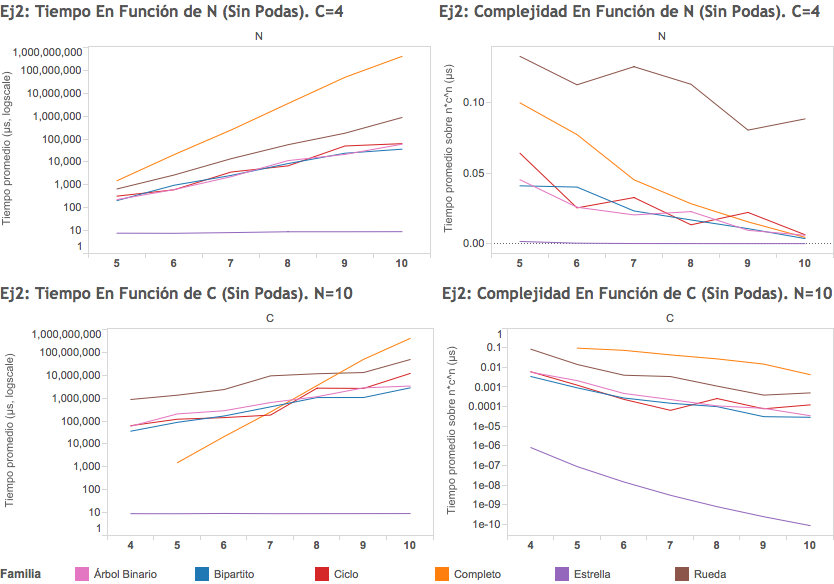
\includegraphics[width=15cm]{grf/TmpEj2}
\caption{Gráficos de tiempo para el ejercicio 2, sin podas}
\label{ex2:time}
\end{figure}
\begin{figure}
\centering
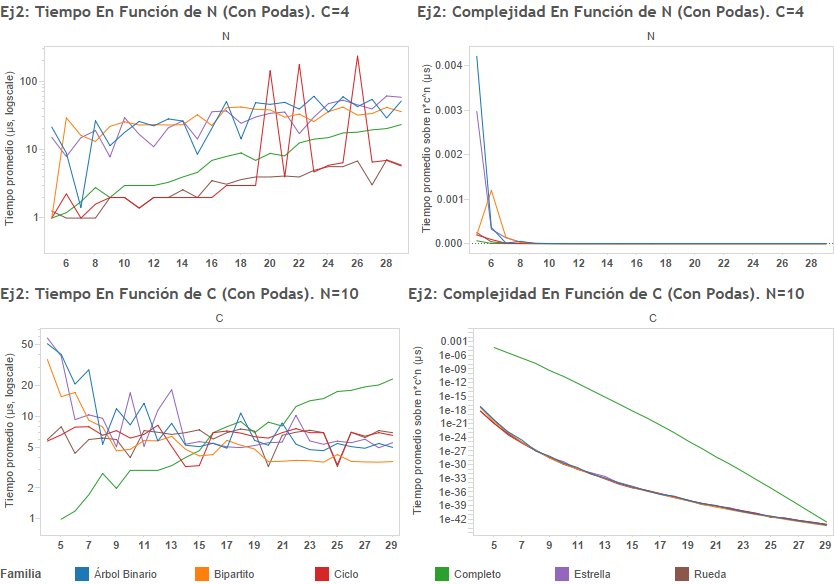
\includegraphics[width=15cm]{grf/TmpEj2Podas}
\caption{Gráficos de tiempo para el ejercicio 2, con podas}
\label{ex2:timepoda}
\end{figure}

Observemos que tanto las figuras \ref{ex2:time} como \ref{ex2:timepoda} muestran que la complejidad es la esperada, ya que los gráficos de complejidad en función de $n$ y de $c$ tienden a constantes, indicando que efectivamente pertenecen a la clase de complejidad mencionada. Cabe destacar la marcada mejoría que nos provee el uso de podas, evidente en la diferencia de escala entre los gráficos con y sin podas. 

\section{Problema 3}

El problema 3 pedía que desarrollemos una heurística golosa para el problema
de list coloring. La heurística que decidimos aplicar es la de ordenar los nodos de manera descendente por grado, y a su vez, ordenar la lista de colores de cada nodo de manera descendente por frecuencia, para luego iterar desde el de mayor grado al de menor, eligiendo el color que menos conflictos generase. Si algún color al momento de ser elegido genera 0 conflictos, se elige ese color para ese vértice y se prosigue al siguiente vértice. 
La idea es que al setear los colores de los nodos de mayor grado con los colores más frecuentes se generasen menos conflictos a futuro y a su vez se minimice la cantidad de colores total a usar.


\begin{figure}
    \centering
    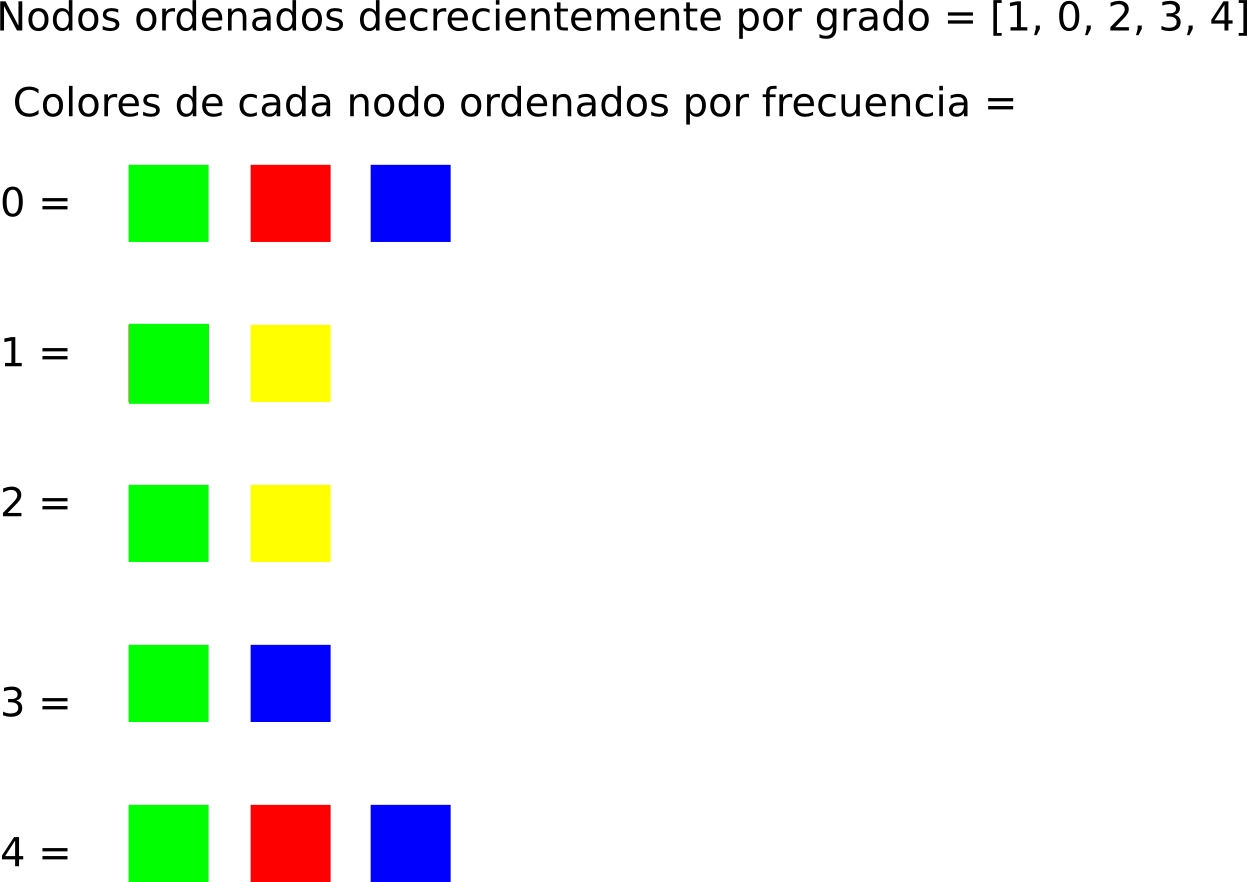
\includegraphics[width=8cm]{examples/3/example3_title.png}
    \begin{minipage}{1\textwidth}
    \hspace*{+0.5cm}
        \begin{tabular}{cccc}
            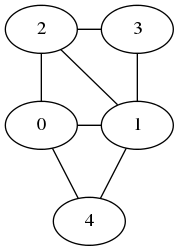
\includegraphics[width=3cm]{examples/3/example3_0.png} &
            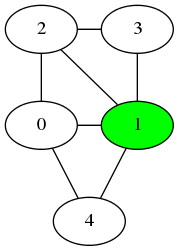
\includegraphics[width=3cm]{examples/3/example3_1.png} &
            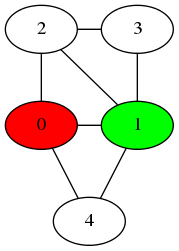
\includegraphics[width=3cm]{examples/3/example3_2.png} &
            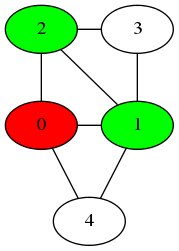
\includegraphics[width=3cm]{examples/3/example3_3.png} \\
            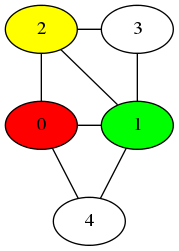
\includegraphics[width=3cm]{examples/3/example3_4.png} &
            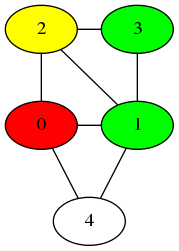
\includegraphics[width=3cm]{examples/3/example3_5.png} &
            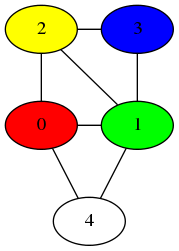
\includegraphics[width=3cm]{examples/3/example3_6.png} &
            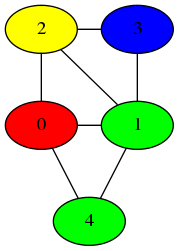
\includegraphics[width=3cm]{examples/3/example3_7.png} \\
            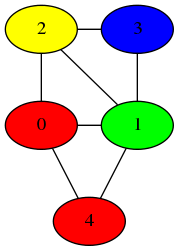
\includegraphics[width=3cm]{examples/3/example3_8.png} &
            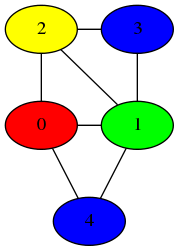
\includegraphics[width=3cm]{examples/3/example3_9.png} 
        \end{tabular}
    \end{minipage}
    \caption{Ejemplo de ejecución de la heurística\label{grf:ex3-example-1}}
\end{figure}


\subsection{Análisis de Complejidad}

La complejidad de la heurística es $O(N^{2}*C + N*C*log(C))$.
Primero, se debe ordenar los colores de cada vértice por su frecuencia global, es decir, cuan frecuentemente aparece ese color en todos los vértices. Esto tiene una complejidad de $O(N*C*log(C))$.
Luego, en la heurística en sí, hay que recorrer $O(N)$ vértices, y por cada vértice, recorrer todos sus colores, ($O(C)$ en peor caso), y a su vez, para cada color, calcular la cantidad de conflictos del vértice con sus vecinos, que pueden ser a lo sumo $O(N)$, lo que nos da una complejidad de $O(N^{2}*C)$.
Finalmente, al sumar la complejidad de realizar el orden por frecuencia y la de la heurística en sí, queda $O(N^{2}*C + N*C*log(C))$ como complejidad de todo el algoritmo.

El caso de un grafo completo es el peor posible, porque todos los nodos tienen que tener un color diferente, siendo la complejidad final $O(N^{2}*C + N*C*log(C))$.

\begin{algorithm}
\caption{Heurística Golosa}
\begin{algorithmic}
\Function{greedyOrder}{graph, colorStorage}
\State colors = colorStorage.sortByFrequency() \Comment $O(N*C*log(C)$
\State vertexOrder = graph.descendingByDegree() \Comment $O(N Log(N))$
\State coloring = ConflictColoring(graph)
\For{v $\in$ vertexOrder}  \Comment $O(N)$
    \State choice = 0
    \State conflicts = $\infty$
    \For{c $\in$ colors[v]}        \Comment $O(C)$
        \State coloring.setu(v, c) \Comment $O(N)$
        \State currentConflicts = coloring.conflicts(v) \Comment $O(1)$
        \If{currentConflicts $<$ conflicts}
            \State choice = c
            \State conflicts = currentConflicts
            \If{currentConflicts $==$ 0}
                \State break
            \EndIf
        \EndIf
    \EndFor
    \State coloring.setu(v, choice) \Comment $O(N)$
\EndFor
\State \Return coloring
\EndFunction
\end{algorithmic}
\end{algorithm}

\begin{algorithm}
\caption{Ordenar colores por frecuencia}
\begin{algorithmic}
\Function{sortByFrequency}{} 
    \State map(UInt, UInt) frequencies
    \State ColorLists colorsByFrequency(colors.size())
    \For{i $\in$ colors} \Comment $O(N)$
        \State colorsByFrequency[i] = list(colors[i]) \Comment $O(C)$
        \For{c $\in$ colorsByFrequency[i]} \Comment $O(C)$
            \If{not(frequencies.find(c))} \Comment $O(log(C))$
                \State frequencies[c] = 1
            \Else
                \State frequencies[c] += 1
            \EndIf
        \EndFor
    \EndFor
    \For {l $\in$ colorsByFrequency} \Comment $O(N)$
        \State l.sort((i, j) $=>$ frequencies[i] $>=$ frequencies[j]) \Comment $O(C * log(C))$
    \EndFor
    \State \Return colorsByFrequency
\EndFunction
\end{algorithmic}
\end{algorithm}

\subsection{Experimentación}


\begin{figure}
\centering
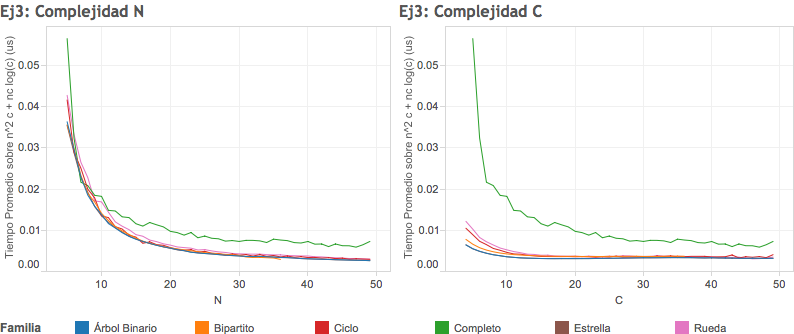
\includegraphics[width=15cm]{grf/Ej3Complexity}
\caption{Complejidad del ejercicio 3 en términos de los valores de N y C para instancias específicas}
\label{grf:ex3comp}
\end{figure}

Como se puede ver en la figura \ref{grf:ex3comp}, el grafo completo es el peor, teniendo la complejidad esperada de $O(N^{2}*C + N*C*log(C))$. Por otro lado, el grafo estrella tiene mucha mejor performance, esto se debe a que el número cromático del mismo es 2, por lo que si todos los vértices tienen al menos 2 colores en común, estos serán los más frecuentes. Por lo tanto, en el momento donde la heurística elige un color para un vértice y se fija la cantidad de conflictos generados, lo que va a pasar es que como mucho tendrá que verificar los 2 primeros colores de la lista de colores del vértice antes de encontrar uno que no genere conflictos. Por esta razón, la complejidad en este caso, y en los casos con un número cromático K conocido, y donde existan los colores necesarios para una solución óptima, la complejidad pasará a ser $O(N^{2}*K + N*C*log(C)) = O(N^{2} + N*C*log(C))$.
El segundo término de la complejidad se mantiene igual sin importar el grafo debido a que consiste en ordenar las listas de colores de los N vértices.

\section{Problema 4}

En términos del problema 4, a priori el algoritmo de búsqueda local es la misma metaheuristica que nos dieron en clase. Como solución inicial tomamos a la solución generada por la heurística del problema 3, y procedemos a realizar la búsqueda local de la forma indicada en clase, visible en el algoritmo \ref{ex4:pseudo1}.

\begin{algorithm}
\caption{Algorítmo de búsqueda local}
\label{ex4:pseudo1}

\begin{algorithmic}
\State current $\gets$ ejercicio3()
\While{1}
    \State next $\gets$ neighbour(current, graph, colors)
    
    \If{current $\leq$ next}
        \State return current
    \Else
        \State current $\gets$ next
    \EndIf
\EndWhile
\end{algorithmic}
\end{algorithm}

Donde la función neighbour nos dice el mejor de los vecinos de la instancia pasada por parámetro. A priori, es claro que este programa termina: dado que neighbour siempre debería devolver al menor de los vecinos, siempre estamos siguiendo una cadena de instancias decrecientes por el criterio de comparación; además, está implícito que todo el conjunto de posibles vecindades de una instancia tiene al menos un mínimo, por lo que eventualmente deberíamos converger hacia el mismo. En términos de las vecindades, optamos por elegir las siguientes heurísticas:

La primer vecindad, visible en el algoritmo \ref{ex4:pseudo2}, considerada consiste en tomar los $k$ vértices con mayor número de colisiones con sus vecinos, y para cada uno de ellos probar con absolutamente todos los colores que no sean el actualmente asignados, tomando como vecino final a aquel cuyo cambio de color genere el menor número de colisiones globales finales. En el caso en que ningún cambio mejore la cantidad de colisiones finales, simplemente nos quedamos con la instancia inicial.

\begin{algorithm}
\caption{Primer vecindad}
\label{ex4:pseudo2}

\begin{algorithmic}
\Function{neighbour}{original, graph, colors}
    \State size $\gets \min(|V(\text{graph})|, k)$ \Comment $O(1)$
    \State conflicts $\gets$ Conflictos por vértice de original \Comment $O(n + m)$
    \State queue $\gets$ min-queue() \Comment $O(1)$
    
    \For{$n \in \{0, .., \text{size}\}$} \Comment $O(k log(k))$
        \State queue.push($\langle$conflicts[$n$], $ n\rangle$) \Comment $O(log(k))$
    \EndFor
    
    \For{$n \in \{\text{size}, .., |V(\text{graph})|\}$} \Comment $O((n - k) log(k))$
        \State current $\gets$ queue.top() \Comment $O(1)$
        
        \If{$\pi_1$(current) $<$ conflicts[$n$]} \Comment $O(1)$
            \State queue.pop() \Comment $O(log(k))$
            \State queue.push($\langle$conflicts[$n$], $ n\rangle$) \Comment $O(log(k))$
        \EndIf
    \EndFor
    
    \State best $\gets$ original \Comment $O(n)$
    
    \For{$n \in \{0, .., \text{size}\}$} \Comment $O(cn + log(k))$
        \State vertex $\gets$ $\pi_2($queue.top()$)$ \Comment $O(1)$
        \State queue.pop() \Comment $O(log(k))$
        \State old $\gets$ color del vértice vertex en el coloreo original \Comment $O(1)$
        
        \For{color admisible para el vértice vertex} \Comment $O(cn)$
            \If{color $\neq$ old} \Comment $O(1)$
                \State next $\gets$ original \Comment $O(n)$
                \State next.set(vertex, color) \Comment $O(n)$
                \If{next.conflicts() $<$ best.conflicts()} \Comment $O(1)$
                    \State best $\gets$ next \Comment $O(n)$
                \EndIf
            \EndIf
        \EndFor
    \EndFor
    
    \Return best
\EndFunction
\end{algorithmic}
\end{algorithm}

La segunda vecindad, en algoritmo \ref{ex4:pseudo2}, consiste en tomar al nodo cuya relación entre cantidad de colisiones con sus vecinos y su grado sea la mayor en todo el grafo, y luego probar con todos los cambios de colores posibles para este nodo, tomando como instancia final aquella que minimice la cantidad de colisiones del nodo elegido con sus vecinos. Una vez más, en el caso en que ningún cambio mejore la cantidad de colisiones finales, simplemente nos quedamos con la instancia inicial.

\begin{algorithm}[h]
\caption{Segunda vecindad}
\label{ex4:pseudo2}

\begin{algorithmic}
\Function{neighbour}{current, graph, colors}
    \State best $\gets$ 0 \Comment $O(1)$
    \State ratio $\gets$ 0 \Comment $O(1)$
    
    \For{$i \in \{0, .., |V(graph)|\}$} \Comment $O(n + m)$
        \State current $\gets$ $\frac{\text{current.conflicts}(i)}{\text{graph.degree}(i)}$ \Comment $O(n + m)$ la primera vez, $O(1)$ luego
        
        \If{current $>$ ratio} \Comment $O(1)$
            \State ratio $\gets$ current \Comment $O(1)$
            \State best $\gets$ i \Comment $O(1)$
        \EndIf
    \EndFor
    
    \State initial $\gets$ current.color(best) \Comment $O(1)$
    \State conflicts $\gets$ current.conflicts(best) \Comment $O(1)$
    
    \For{color $\in$ colors.get(best)} \Comment $O(cn)$
        \If{color $\neq$ initial} \Comment $O(1)$
            \State previous $\gets$ current.color(best) \Comment $O(1)$
            \State current.set(best, color) \Comment $O(n)$
            
            \If{current.conflicts(best) $<$ conflicts} \Comment $O(1)$
                \State conflicts $\gets$ current.conflicts(best) \Comment $O(1)$
            \Else
                \State current.set(best, previous) \Comment $O(n)$
            \EndIf
        \EndIf
    \EndFor
    
    \Return current
\EndFunction
\end{algorithmic}
\end{algorithm}

Cabe destacar que en el caso de la primera heurística el criterio que determina la mejoría de una instancia con respecto a otra es la cantidad de colisiones a nivel global (a pesar de que el cambio sea a nivel local), mientras que en el caso de la segunda es la cantidad de colisiones del nodo contra sus vecinos, que es un criterio local. Como criterio de comparación entre instancias, decidimos tomar el indicador que nos resultó más natural para determinar qué tan buena es una instancia: la cantidad de colisiones a nivel global. Esto quiere decir que en cada paso, la búsqueda local sólo puede mejorar la solución en términos de cantidad de colisiones globales, garantizándonos de esta forma que al finalizar poseemos un mínimo local bajo este criterio.

En términos de la implementación, dado que en este caso necesitamos acceder muy frecuentemente a información sobre los conflictos a nivel global y entre vecinos, utilizamos una representación con información sobre la cantidad de conflictos de cada vértice con el coloreo actual, y cambiamos las operaciones para que cada actualización del coloreo mantenga actualizada esta información adicional de manera acorde.

\subsection{Análisis de Complejidad}

Es importante hablar primero sobre la implementación de un coloreo que realizamos: originalmente, la estructura de un coloreo consistía básicamente en un arreglo con una asociación de colores para cada nodo y un valor reservado particular que indicaba la falta de un color en los casos en que fuera necesario. Sin embargo, la gran cantidad de cálculos con respecto a la cantidad de conflictos que presentaban las heurísticas nos hicieron considerar una alternativa ligeramente más sofisticada: en la implementación actual, poseemos además un arreglo que indica la cantidad de colisiones de cada nodo con sus vecinos, así como una variable que cuenta la cantidad de colisiones a nivel global, y una variable adicional que indica si el arreglo está actualizado. Esta representación nos permite garantizar una complejidad temporal de $O(1)$ al obtener los conflictos cuando el arreglo está actualizado, y nos fuerza a realizar una actualización (que nos toma $O(n + m)$) en los casos en que no lo está. Además, agregamos una variante de la operación de coloreo que nos permite realizar la actualización al momento en que se realiza la operación, costando un total de $O(dg(v)) = O(n)$ en el peor caso.

\begin{figure}
    \centering
    \begin{minipage}{0.29\textwidth}
        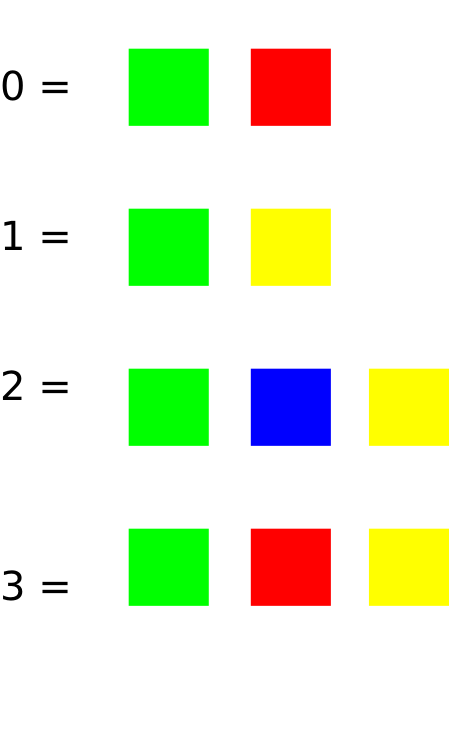
\includegraphics[width=3cm]{examples/4/1/example4_1_title.png}
    \end{minipage}
    \begin{minipage}{0.70\textwidth}
        \begin{tabular}{ccc}
            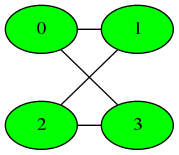
\includegraphics[width=3cm]{examples/4/1/example4_1_0.png} &
            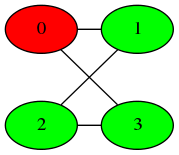
\includegraphics[width=3cm]{examples/4/1/example4_1_1.png} &
            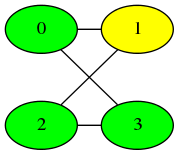
\includegraphics[width=3cm]{examples/4/1/example4_1_2.png} \\
            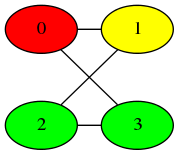
\includegraphics[width=3cm]{examples/4/1/example4_1_3.png} &
            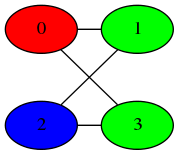
\includegraphics[width=3cm]{examples/4/1/example4_1_4.png} &
            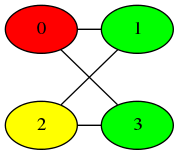
\includegraphics[width=3cm]{examples/4/1/example4_1_5.png}
        \end{tabular}
    \end{minipage}
    \caption{Ejemplo de corrida de la primera vecindad cuando se toma $k=2$, donde los pasos suceden desde la esquina superior izquierda hacia la inferior derecha. \label{grf:ex4-example-1}}
\end{figure}

En el caso de la primera vecindad, no es muy complicado el análisis de complejidad: los primeros dos ciclos acumulan un total de $O(n log(k))$ pasos en conjunto, y el último de los ciclos basta con ver el código para encontrase con que la complejidad es $O(cn + nlog(k))$, haciendo que en total tengamos $O(n(c + log(k)))$ tras considerar todas las operaciones.

\begin{figure}
    \centering
    \begin{minipage}{0.19\textwidth}
        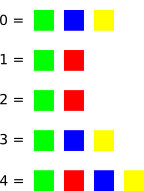
\includegraphics[width=3cm]{examples/4/2/example4_2_title.png}
    \end{minipage}
    \begin{minipage}{0.80\textwidth}
        \begin{tabular}{ccc}
            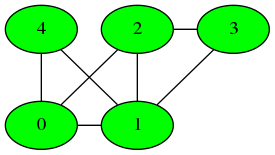
\includegraphics[width=4cm]{examples/4/2/example4_2_0a.png} &
            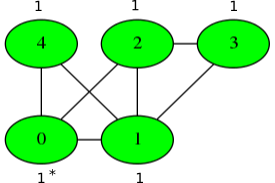
\includegraphics[width=4cm]{examples/4/2/example4_2_0b.png} &
            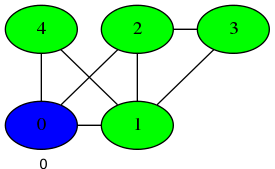
\includegraphics[width=4cm]{examples/4/2/example4_2_1.png} \\
            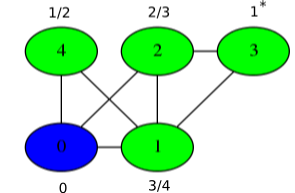
\includegraphics[width=4cm]{examples/4/2/example4_2_2.png} &
            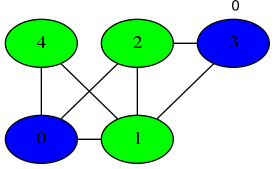
\includegraphics[width=4cm]{examples/4/2/example4_2_3.png} &
            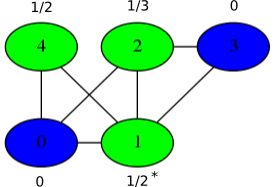
\includegraphics[width=4cm]{examples/4/2/example4_2_4.png} \\
            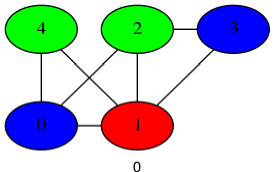
\includegraphics[width=4cm]{examples/4/2/example4_2_5.png} &
            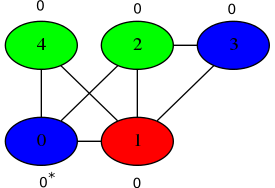
\includegraphics[width=4cm]{examples/4/2/example4_2_6.png} &
            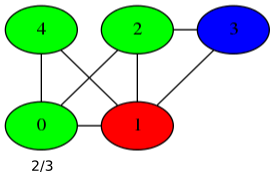
\includegraphics[width=4cm]{examples/4/2/example4_2_7.png} \\
            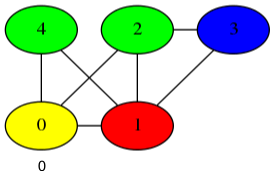
\includegraphics[width=4cm]{examples/4/2/example4_2_8.png}
        \end{tabular}
    \end{minipage}
    \caption{Ejemplo de corrida de la segunda vecindad, donde los pasos suceden desde la esquina superior izquierda hacia la inferior derecha. Los números mostrados arriba de los nodos se corresponden con el coeficiente del nodo en la corrida, y las marcas con asterisco al nodo elegido para cambiar el color en la corrida. \label{grf:ex4-example-1}}
\end{figure}

En el caso de la segunda vecindad, tomar el grado de un nodo es una operación $O(1)$ y todas las otras realizadas en el primer ciclo también lo son. Por lo que la complejidad temporal es $O((n + m) + (n - 1)) = O(n + m)$ para el primer ciclo, donde el primer término proviene de la primer iteración, y el segundo de todas las otras juntas. Luego, en términos del segundo ciclo, el mismo se realiza a lo sumo $c$ veces, y en el peor caso ningún cambio de color mejora la cantidad de conflictos, por lo que terminamos realizando $O(2n) = O(n)$ operaciones en cada iteración, por un total de $O(cn)$ en todo el ciclo. Finalmente, la complejidad del algoritmo para obtener el mejor vecino es $O(n + m + cn) = O(cn + m)$ (aunque cabe destacar que en realidad ese $O(cn)$ es una cota grosera para la complejidad real, que es $O(c * dg(best))$; pensamos que esta cota más ajustada podría servirnos cuando realicemos el análisis de mejor y peor caso con hipótesis adicionales sobre los grados de los nodos).

Pensemos, entonces, qué sucede con la búsqueda local. En el mejor caso, el resultado del ejercicio 3 es un mínimo local de antemano, en cuyo caso vamos a estar ejecutando una única vez la iteración de la búsqueda, encontrando que no hay mejoría y saliendo de esta forma. En el peor caso, el resultado del ejercicio 3 tiene exactamente $m$ conflictos (es el caso en el que todos los nodos tienen el mismo color), y asumiendo que bajamos de a exactamente un conflicto hasta llegar al óptimo de cero conflictos, tenemos exactamente $m$ iteraciones de la vecindad. Por lo tanto, en el peor caso tendríamos $O(mn(c + log(k)))$ para la búsqueda local con la primer vecindad, y $O(m(cn + m))$ para la segunda vecindad.

\section{Conclusiones Heuristicas}

Encontramos, principalmente, que la heurística constructiva tiende a generar soluciones sin conflictos para grafos con estructura adicional, como los grafos completos, bipartitos, y demás familias con las que experimentamos. Además, una mirada rápida al comportamiento de las instancias aleatorias nos reveló que los grafos aleatorios que tenían una cierta cantidad de conflictos tendían a no mejorar ampliamente al aplicar la búsqueda local; sino que no encontramos diferencias de más de 40 colisiones menos.

Sospechamos que esto sucede porque los grafos en los que sucede esto tienen problemas en el coloreo que son más graves que un nodo, sino que hay un conjunto de nodos vecinos en conflicto, que es un caso no explorado por nuestras heurísticas. Sospechamos que heurísticas que miren conjuntos de nodos vecinos podrían mejorar ampliamente estos casos.

Observando la figura \ref{grf:heu}, es fácil ver que efectivamente sucede esto mencionado anteriormente sobre la mejoría de las heurísticas de búsqueda local contra la golosa. A su vez, la heurística 4A, que trata de minimizar conflictos más a nivel global resulta generar menos conflictos que 4B, que está un poco más enfocada en los vecinos de un nodo que los conflictos a nivel global, para así tratar de reducir la cantidad de conflictos. Suponemos que esta diferencia se da ya que la segunda búsqueda se orienta más a resolver conflictos locales, por lo que es posible que quede encerrada en mínimos locales. La primer búsqueda, por el contrario, al tratar de reducir los conflictos de una manera más global, parece no caer tanto en ese problema.

Además, los gráficos dejan claro las relaciones que se dan entre las distintas variables: una mayor cantidad de colores disponibles tienden a hacer que tengamos menor cantidad de colisiones, y una mayor cantidad de aristas tiende a tener el mismo efecto. Si bien estas relaciones son intuitivas (y están claramente motivadas porque menos colores y más aristas implican más restricciones), es interesante que se reflejen tan claramente en los gráficos. Más aun, observemos cómo inclusive con una gran cantidad de nodos y aristas, tener muchos colores baja efectivamente las restricciones hasta hacer que sea posible colorear sin conflictos.

\begin{figure}
\centering
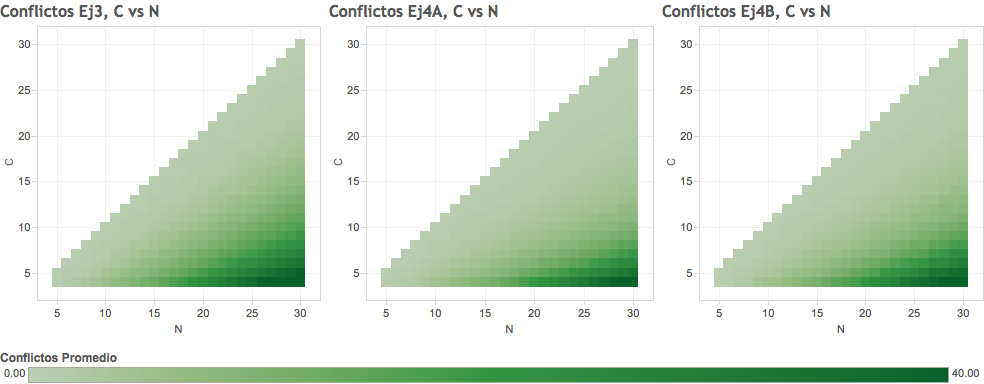
\includegraphics[width=15cm]{grf/ConflictosCvsN.png}
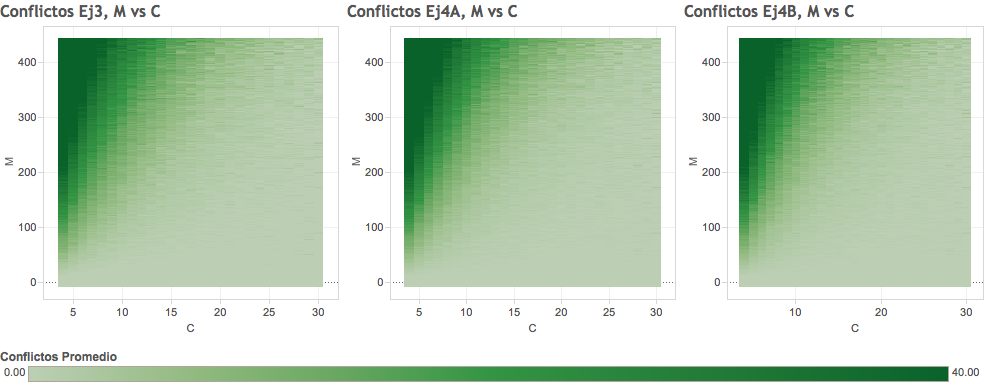
\includegraphics[width=15cm]{grf/ConflictosMvsC.png}
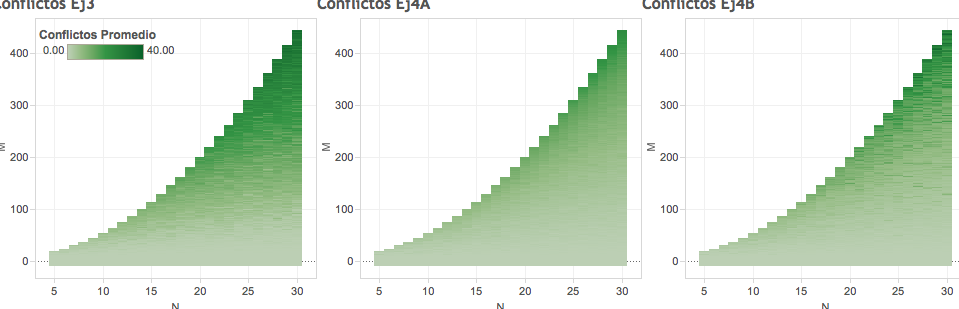
\includegraphics[width=15cm]{grf/ConflictosNvsM.png}
\caption{Gráficos de cantidad de conflictos promedio sobre grafos generados aleatoriamente en términos de C, N y M. Un color más oscuro indica mayor cantidad de conflictos promedio.}
\label{grf:heu}
\end{figure}

\end{document}